\documentclass[12pt,titlepage]{article}
\usepackage[ngerman]{babel}
\usepackage[utf8]{inputenc}
\usepackage{color}
\usepackage[a4paper,lmargin={2cm},rmargin={2cm},tmargin={2.5cm},bmargin = {2.5cm}]{geometry}
\usepackage{amssymb}
\usepackage{amsthm}
\usepackage{graphicx}
\title{
\includegraphics{images/arc42-logo.png}}
\author{Jawoon Kim, Charlie Wiegand}
\begin{document}
    \begin{titlepage}
    \centering
    
\includegraphics[width=0.3\textwidth]{images/arc42-logo.png}\par\vspace{1cm}
    {\scshape\LARGE bib International College\par}
    \vspace{1cm}
    {\rmfamily\scshape Lernaufgabe 2020\par}
    \vspace{1.5cm}
    {\Huge\bfseries bib now\par}
    \vspace{2cm}
    {\Large\itshape Charlie Wiegand\par Jawoon Kim\par}
    \vfill
    betreut von Frau Langeheinecke\par
    \vfill
    {\large \today\par}
    \end{titlepage}

\tableofcontents
\newpage

\maketitle

\addcontentsline{toc}{section}{Abbildungsverzeichnis}
\listoffigures

\pagebreak

\section{Über bibnow}



\section{Aufgabenstellung}


\textbf{Inhalt.}

Da zur Zeit häufig Mails an die ganze Schule geschickt werden, wenn beispielsweise jemand etwas verloren hat, wollen wir unseren Mitschülern und uns ein Forum bieten, das diesen Austausch erleichtert.

Für dieses Vorhaben haben wir uns folgende Ziele und Richtlinien gesetzt

\begin{itemize}
\item
\textbf{Minimum}
  Es soll eine lauffähige Webseite erstellt werden, auf der man sich mindestens einloggen kann und anschließend Beiträge in Textform hochladen kann. 
\item
\textbf{Optional}
  Es soll die Möglichkeit geben seine Beiträge durch Bilder zu ergänzen und die Posts sollen in Kategorien eingeteilt werden
\item
\textbf{Optional}
Desweiteren soll es die Möglichkeit den Stundenplan und Klausurplänung aus dem offiziellen Intranet zu übernehmen.

\end{itemize}


\textbf{Vorausetzungen}
Um das Minimum zu erreichen benötigen wir einen PC, einen Texteditor, npm, ein AngularFramework und Firebase. Um uns die Zusammenarbeit zu erleichtern haben wir uns entschieden Versionskontrolle über git laufen zu lassen und die Ergebnisse über GitHub auszutauschen. 

\newpage
\section{Konzepte}

\subsection{Inhaltskonzept}

\vspace{2cm}

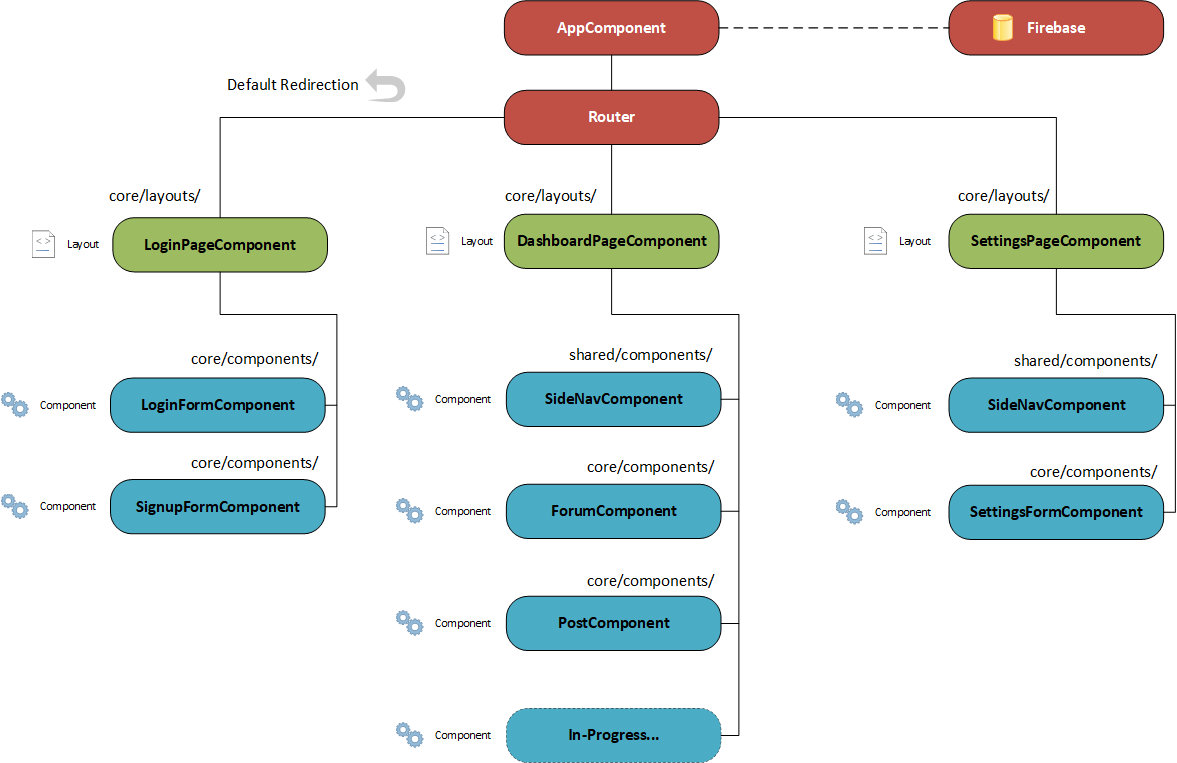
\includegraphics[width=400pt]{Konzepte/bibnow_Sitemap.png}


\vspace{2cm}

Bei bib-now handelt es sich um ein Schülerforum für das bib international College Paderborn. Die technische Umsetzung basiert auf  einer Single-Page-Webanwendung mit einer RealTime-Datenbank deren einzelnde Komponenten über einen Router verlinkt sind: Die Navigation besteht aus drei Komponenten: LoginPageComponent, DashboardPageComponent und der SettingsPageComponent. Jede dieser Komponenten besitzt ihre eigenen Backend-Komponenten. Die LoginPage greift auf die LoginFormComponent und SignUpFormComponent zurück. Die DashboardPageComponent greift auf  SideNavComponent, ForumComponent, PostComponent zurück. Außerdem könnnen hier später weitere Elemente ergänzt werden. SettingsPageComponent beinhaltet die SideNavComponent und SettingsFormComponent. 


\pagebreak

\subsection{Navigationskonzept}

\vspace{2cm}

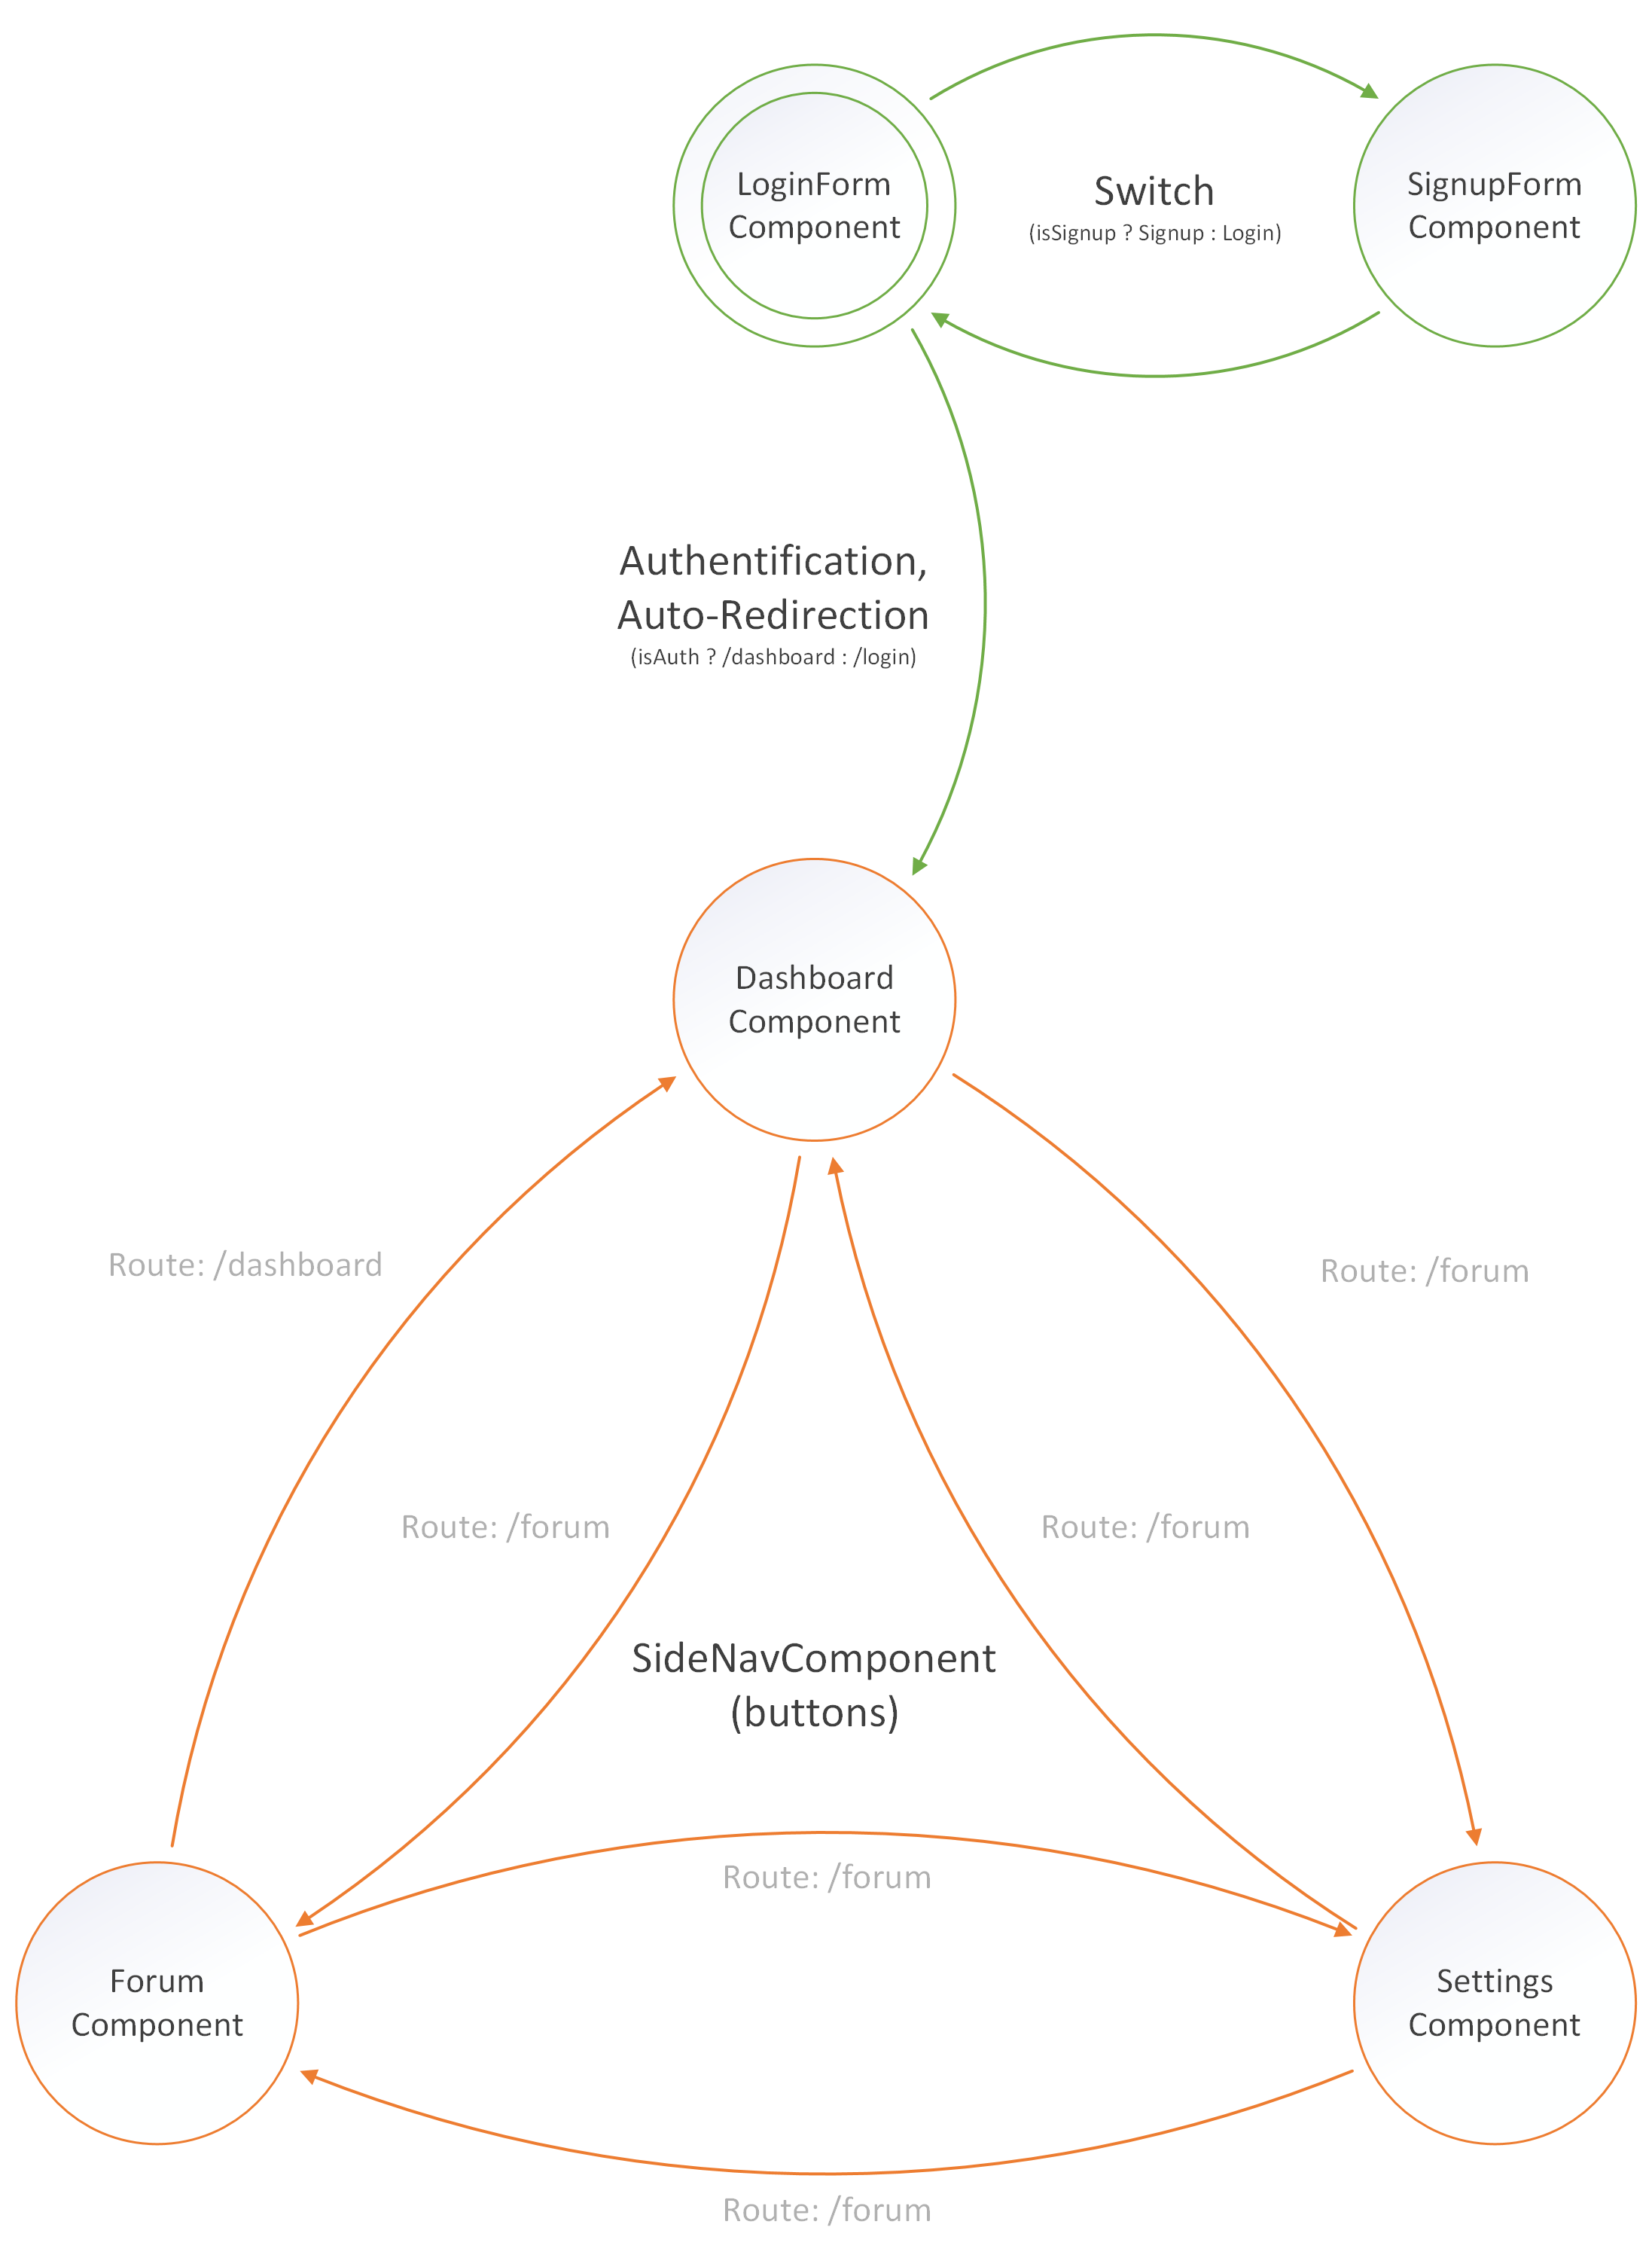
\includegraphics [width=400pt]{Konzepte/bibnow_Navigationskonzept}



\vspace{2cm}


Beim Betreten der Seite wird der User zunächst aufgefordert sich einzuloggen. Sollte er sich noch nicht registriert haben hat er die Möglichkeit in das Registrierungsforumlar zu switchen und sich dort zu registrieren. War die Registrierung oder das einloggen erfolgreich, wird der User auf die DashboardPage weitergeleitet. Dort werden ihm Posts angezeigt und er hat die Möglichkeit über ein Formular einen eigenen Post zu verfassen. Außerdem kann er über das Navigationsmenu zu der SettingsPage zu wechseln. Seine aktuelle Position wird durch eine Farbveränderung am jeweiligen punkt in der Navigatonsleiste erkenntlich.

\newpage
\subsection{Gestaltungskonzept}

Font: Montserrat (https://fonts.google.com/specimen/Montserrat)
Font Weights: 100, 300, 700
\vspace{2cm}
\begin{itemize}
\item
	Für Subtitel, gedämpfte Texte, etc


\includegraphics{images/Schriftart_100.png}
\item
	Für normale Texte, Standard-schriftart


\includegraphics{images/Schriftart_300.png}
\item
	Für Titel und Akzent(Betonung)


\includegraphics{images/Schriftart_700.png}
\end{itemize}


Farbenschema

Schemakonzept: Neon + Material

Primärfarbe:\#D43D61

Sekundär:\#039BE5

Hintergrund:\#271D33

Hintergrund Beiträge:\#F8F6F6

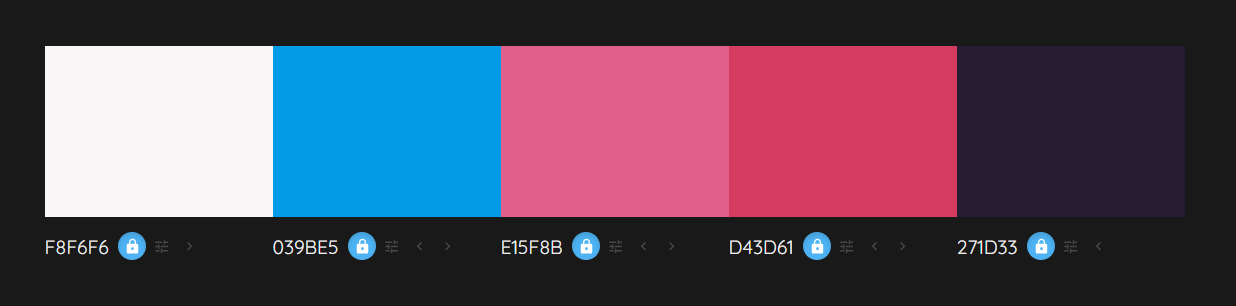
\includegraphics[width=400pt]{images/Schema_1.png}

\subsection{Zielgruppendefinition}

Aus den MUSS - und KANN-Zielen ergibt sich unsere Zielgruppe: alle Schüler und Mitarbeiter des bib international College Paderborn. 


\section{Durchführung}

\subsection{Allgemeine Beschreibung zur Durchführung}

Beim Entwickeln der Webseite  haben wir uns täglich Abgesprochen welche Features wir als nächstes brauchen und diese in Form von  Backend und Frontend unter uns aufgeteilt. Da wir über GitHub gearbeitet haben konnten wir beide unsere branches pushen und mit dem Master-Branch auf konfliktfreie Kompatibiltät prüfen und anschließend testen.

\subsection{Planung und Vorbereitung}

\subsubsection{Vor dem Projekt}

Corona bedingt wurden wir erst recht spät über die LEA informiert. Wir haben die Zeit die wir dennoch noch zur Vorbereitung hatten, genutzt um uns über Nutzung des Frameworks Angular sowie die dortige implementierung von Firebase Funktionen zu informieren. Dies geschah in Form von diversen Youtube-Videos sowie dem Durchstöbern der jeweiligen Dokumentationen.\\ \\
Wir sind davon ausgegangen, dass wir eine lauffähige Webseite mit den minimal Anforderungen in den ersten Tagen realisieren können und uns anschließend mit den optionalen Zielen und der Dokumentation beschäftigen können.

\subsubsection{Während des Projekts}

Zu Beginn haben wir die Dateistruktur sowie den Ablauf abgesprochen. Wir haben uns darauf geeinigt, dass wir die Anwendung der Seite zurnächst in Core und Shared unterteilen. Der Core-Ordner soll außerdem in Components und Layouts unterteilt werden, um eine physische Trennung von Logik und Frontend zu erzielen. Der Shared-Ordner soll alle restlichen Komponenten enthalten unterteilt in ihre jeweilen Oberkategorien: Models, Guards, Services, Module und Components die in das Core Modell integriert werden. \\ \\






\section{Ergebnis}

\subsection{GitHub-Pfad}

Der Source-Code zum Ergebnis lässt sich unter folgendem Github Repository https://github.com/bib-lea/bib-now
finden.

%TODO Ergebnis

\section{Fazit}
x

\section{Quellen}

\section{Literaturverzeichnis}


\end{document}
 
